\chapter{A certificate that contains an actual field}
\label{chap:g07-certificate}

\section{What an inverse construction must return}

The preceding chapters provide several exact objects attached to a finite group. A multiplication table determines the group. Its regular representation determines a family of rational permutation matrices. Its subgroups determine averaging projectors. The variable construction supplies a finite Galois extension over an invariant field. Each output has a definite mathematical type. The inverse Galois target requires a finite field over $\Q$.

One useful way to express the remaining task is to specify a certificate that would finish it for a chosen group. The specification makes no assertion that the certificate is easy to find. It states what a proposed construction must contain before the arithmetic conclusion follows.

Let $G$ be a finite group of order $n$. A polynomial field presentation consists of a monic irreducible polynomial $f\in\Q[X]$ of degree $n$ and
\[
 L=\Q[X]/(f),\qquad \theta=X\bmod f.
\]
Irreducibility is the field input. The quotient is automatically a commutative algebra of dimension $n$, but that dimension alone would also hold for a reducible polynomial. A reducible quotient can have zero divisors or nilpotents and cannot serve as the requested field.

For every $g\in G$, specify a polynomial $r_g\in\Q[X]$ of degree less than $n$. It is intended to describe $\sigma_g(\theta)=r_g(\theta)$. The equality
\[
 f(r_g(\theta))=0
\]
ensures that this substitution induces a unital $\Q$-algebra endomorphism of $L$. Because $L$ is a field, the endomorphism is injective. Because it is a linear endomorphism of a finite dimensional vector space, it is surjective. Thus it is an automorphism.

The group law must still hold. With our convention that $\sigma_g\sigma_h$ means apply $\sigma_h$ first, the required congruences are
\begin{align}
 r_1(X)&\equiv X\pmod f,\label{eq:g07-unit}\\
 r_h(r_g(X))&\equiv r_{gh}(X)\pmod f.\label{eq:g07-composition}
\end{align}
The reversed order of the displayed polynomial substitutions is deliberate. Applying $\sigma_g$ to $r_h(\theta)$ replaces $\theta$ by $r_g(\theta)$, since rational coefficients are fixed. Finally the residues $r_g\bmod f$ must be pairwise distinct. Equal generator images would give equal automorphisms and could collapse the intended group.

\begin{theorem}[Finite field realization certificate]
\label{thm:g07-certificate}
Suppose $f$ and $(r_g)_{g\in G}$ satisfy the field, root, composition and distinctness conditions above. Then $L/\Q$ is finite Galois and
\[
 \Gal(L/\Q)\simeq G.
\]
\end{theorem}

\begin{proof}
The substitutions give a homomorphism from $G$ into $\Aut_{\Q}(L)$. The identity and composition congruences prove the homomorphism law. Distinct generator images make the homomorphism injective. Write its image as $\Sigma$, so $|\Sigma|=n$.

Apply the finite automorphism fixed-field theorem, in the form recorded in source contract LC10. It gives a finite Galois extension $L/L^\Sigma$ with
\[
 [L:L^\Sigma]=|\Sigma|=n,
 \qquad \Gal(L/L^\Sigma)=\Sigma.
\]
All substitutions fix $\Q$, hence $\Q\subseteq L^\Sigma$. Since $[L:\Q]=\deg f=n$, the degree formula gives
\[
 n=[L:L^\Sigma][L^\Sigma:\Q]
   =n[L^\Sigma:\Q].
\]
Therefore $L^\Sigma=\Q$. The preceding Galois assertion now has the required rational base, and the full group is $\Sigma\simeq G$.
\end{proof}

The theorem is a sufficient certificate, not a restriction on what a genuine realization may look like. Every finite Galois extension in characteristic zero has a primitive element. A realization of $G$ has degree $|G|$, and each automorphism's image of that element has a unique expression in the power basis. Thus an existing realization can be written in this format. The primitive element theorem is the classical input, rather than a new search procedure \cite[Theorem 5.1]{Milne2022}.

\section{An exact quadratic certificate}

For $G=C_2=\{1,s\}$, take $f=X^2-2$ and choose
\[
 r_1=X,\qquad r_s=-X.
\]
The polynomial is irreducible over $\Q$, because two is not a rational square. Both residues satisfy $f(r_g)\equiv0\pmod f$. The nontrivial composition gives $r_s(r_s(X))=X$, and the two images are distinct. The certificate theorem returns $\Q(\sqrt2)/\Q$ with its full group $C_2$.

This example shows why the certificate has several checks. The substitution $r_s=X$ would still preserve the polynomial but would fail distinctness. The same pair of substitutions with $f=X^2-1$ would pass root and composition calculations but fail the field condition. One cannot replace irreducibility by an appealing symmetry of the roots.

\section{The multiplication carried by a normal basis}

The normal basis theorem supplies a regular module for an already existing finite Galois extension \cite[Theorem 5.18]{Milne2022}. If $L/\Q$ has group $G$ and normal basis generator $\alpha$, the vector-space map
\[
 \Phi:\Q[G]\longrightarrow L,
 \qquad \sum_g a_g g\longmapsto\sum_g a_g g(\alpha)
\]
is an equivariant linear isomorphism. It transfers subgroup averages and their fixed vector spaces. It is not a claim that the usual multiplication in $\Q[G]$ is field multiplication.

The transported multiplication is a bilinear map
\[
 \mu:\Q[G]\otimes_\Q\Q[G]\longrightarrow\Q[G],
 \qquad \mu(u,v)=\Phi^{-1}(\Phi(u)\Phi(v)).
\]
For the left regular action $\lambda$, it obeys
\[
 \lambda(g)\mu(u,v)=\mu(\lambda(g)u,\lambda(g)v).
\]
It is associative and commutative, has a unit and has no zero divisors. Its coefficients depend on the field and on the chosen normal basis. The normal basis theorem assumes that field before producing the basis. It cannot be used backwards to infer that an arbitrary choice of these coefficients has all the required properties.

The coordinate algebra $\Q^G$ provides a precise comparison. Its pointwise product is equivariant under regular translation, associative, commutative and unital. The invariant subalgebra consists of constant functions, so it is $\Q$. Nevertheless, two different coordinate idempotents multiply to zero. This algebra satisfies many visible symmetry and fixed-object conditions while failing the field condition. For a nontrivial $G$, it is a disconnected algebra rather than a number field.

A coordinate construction must supply a rational multiplication tensor defining a field, verify that the prescribed action preserves it, and identify the full rational automorphism group. The certificate above records these obligations.

\begin{figure}[tbp]
\centering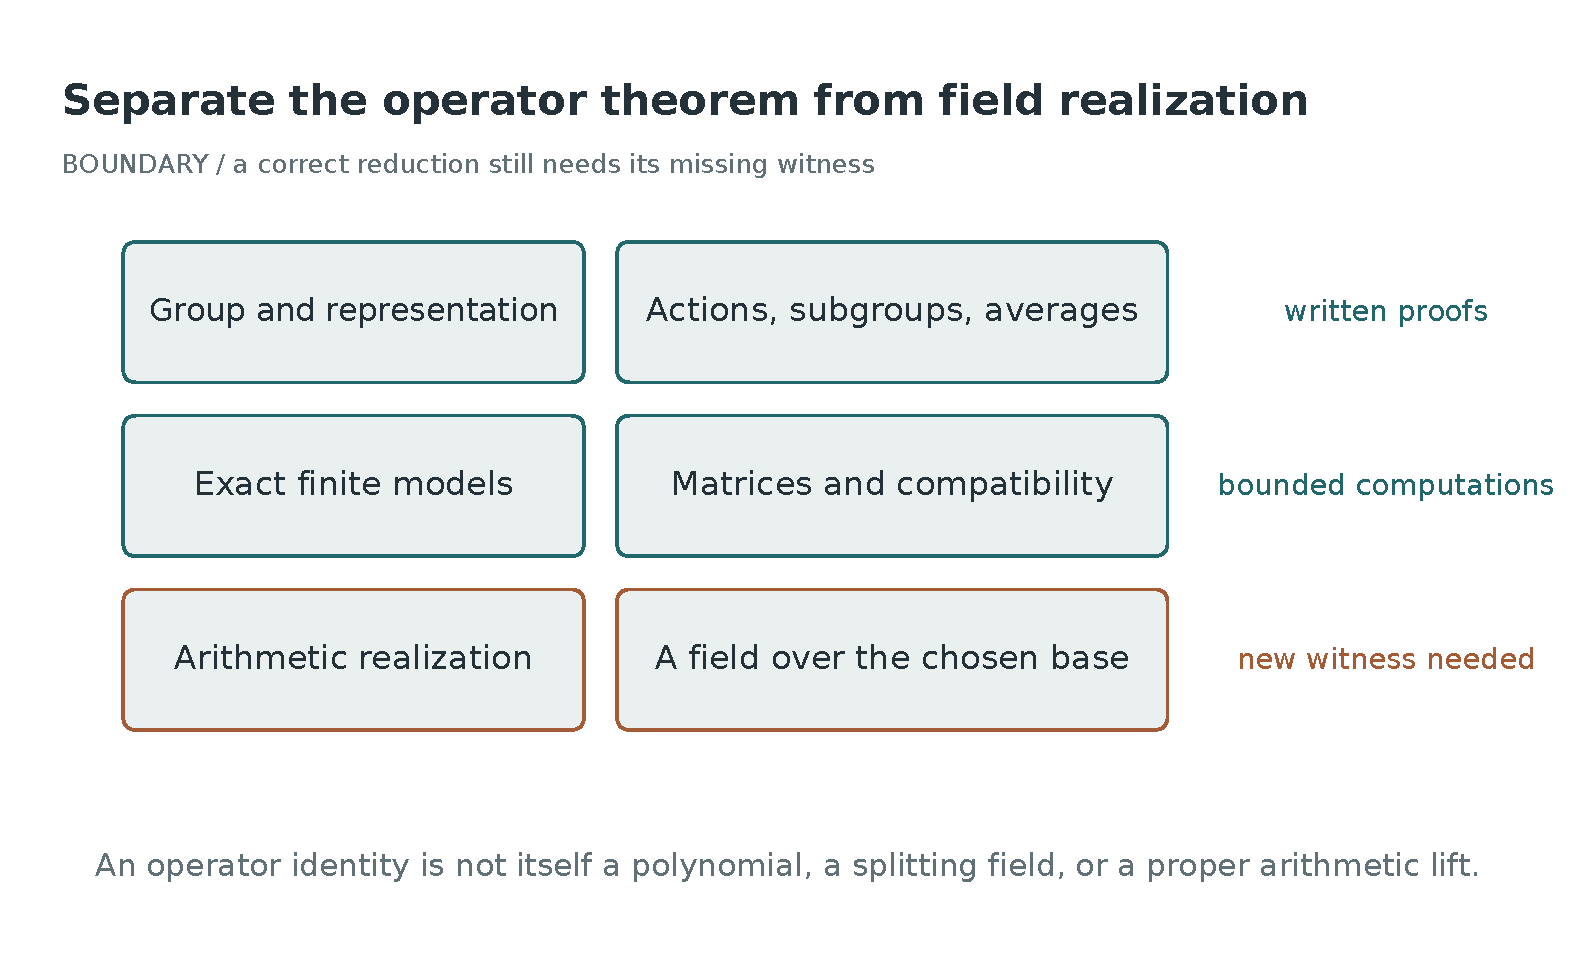
\includegraphics[width=0.85\linewidth]{../visual/figures/20_boundary.pdf}
\caption{Finite symmetry can describe different objects. The inverse Galois target requires a number field over $\Q$ with exactly the prescribed full automorphism group.}
\label{fig:g07-boundary}
\end{figure}

\section{Finding and verifying are different tasks}

Given rational candidates, root and composition tests use exact polynomial remainders, and distinctness uses reduced residues. Irreducibility still needs an exact field certificate, for example a suitable modular argument.

These checks can reject a reducible quotient, a collapsed action or an incorrect fixed base. Passing them for one group does not construct candidates for every group or give a uniform time or size bound.

The finite checks cover five polynomials, all 36 ordered pairs of six $S_3$ subgroups, a faithful $S_4$ boundary and two lift models. Their scope is these examples.

\chapter{The remaining realization program}
\label{chap:g08-program}

\section{What this edition closes}

The five field examples are complete realizations of their specified groups. Their proofs account for field degree, separability and the full splitting-field group. The projector arguments are universal statements in their declared regular representation. The finite lifting examples distinguish compatibility from properness. The certificate theorem turns explicit rational field data into a full realization statement.

The larger uniform routes remain conditional at identifiable points. The variable action realizes every finite group over its invariant field. A rational parametrization of that invariant field would allow Hilbert specialization. A regular realization over $\Q(t)$ would also supply an arithmetic realization. An existing quotient of the absolute Galois group can be lifted only when the specified embedding problem has an appropriate continuous proper solution.

These are useful reductions because they identify the objects and maps a proposed argument must construct. None is an implication from a bare regular matrix representation to a number field. The representation calculus preserves and exposes structure that has been supplied. An inverse existence theorem must supply the arithmetic structure as well.

\section{Classical sectors and dated external work}

The solvable sector has an external existence theorem. In the corrected proof source of Schmidt and Wingberg, every finite solvable group occurs over every global field, in particular over $\Q$ \cite[Theorem 1]{SchmidtWingberg1998}. This is a theorem of classical inverse Galois theory. The cited statement does not promise arbitrary prescribed local completions, a discriminant bound or a polynomial-time construction. Those extra conclusions would require extra arguments.

Symmetric groups also admit classical rational realizations \cite[Example 4.32]{Milne2022}. The quartic calculation in this reader is one explicit instance. Its exact modular factors become useful only through the good-prime cycle theorem and the subgroup argument. The general construction should retain monicity when coefficients are assembled by the Chinese remainder theorem. The source contracts record a presentation correction in the printed example, rather than silently copying a polynomial whose leading coefficient is wrong.

The source check for this edition includes the October 2026 version of the $M_{23}$ preprint by Huang, Jackson, Lee, Poonen, Pries and Zhang \cite{HuangEtAl2026}. Its stated theorems give both a rational and a regular realization of that group. We use that result as dated external context. We have not reproduced its Belyi-map calculations or independently checked its Magma certificates. It is not a dependency of the elementary arguments here. It also does not settle the problem for every finite group.

\begin{figure}[tbp]
\centering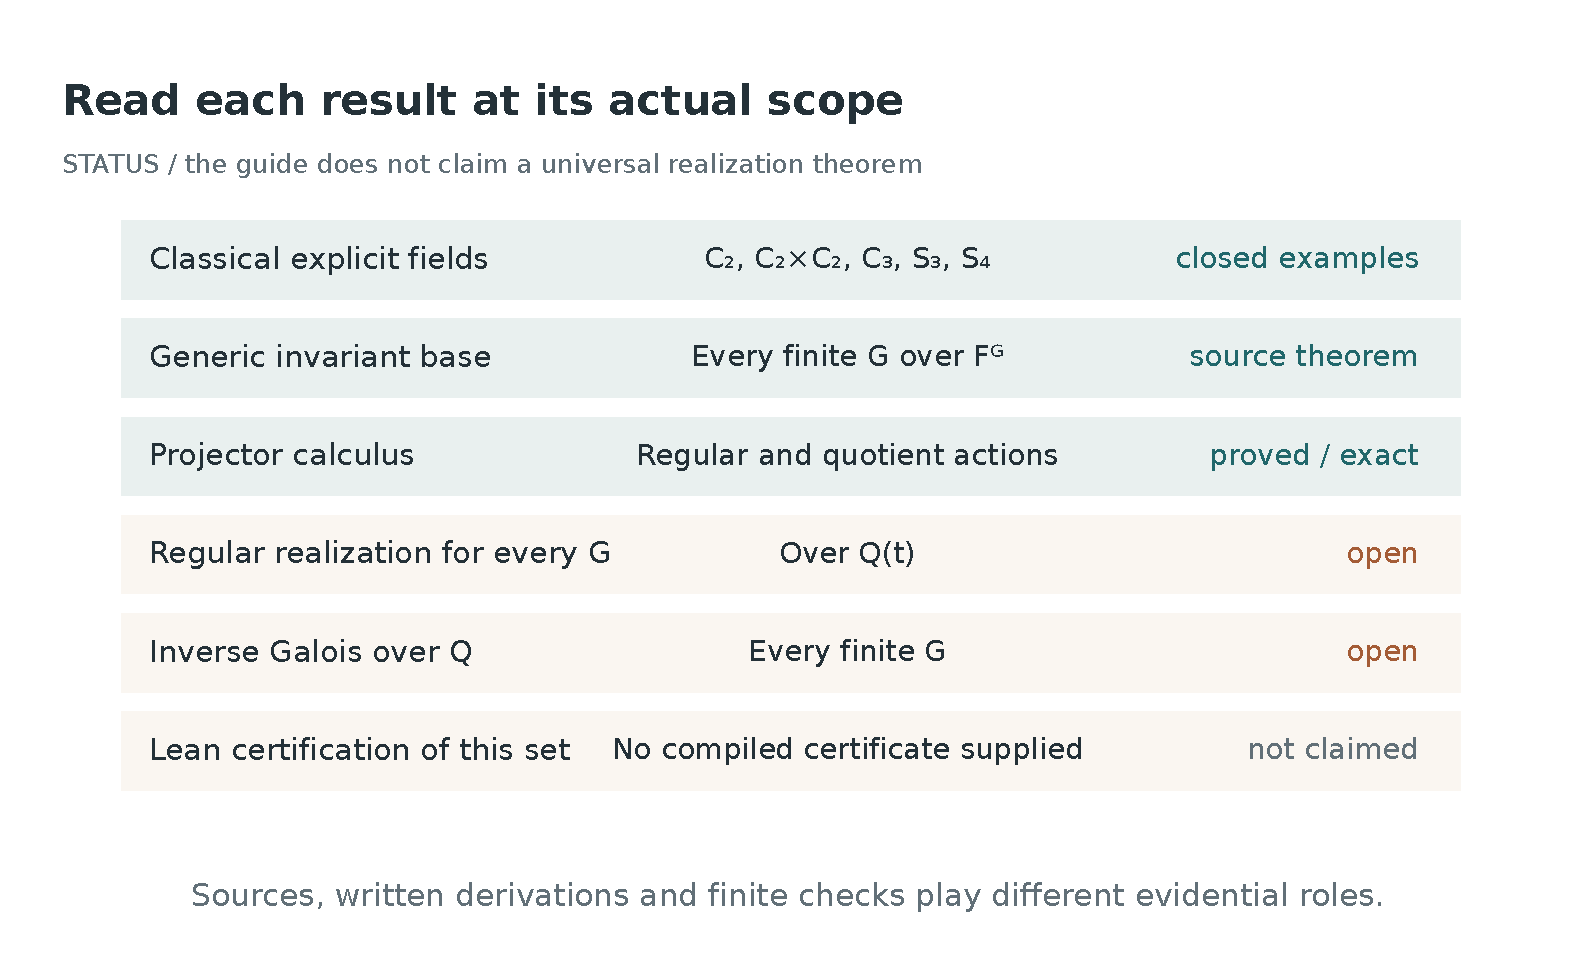
\includegraphics[width=0.94\linewidth]{../visual/figures/21_status_map.pdf}
\caption{Evidence has several roles. Written project arguments, external classical existence theorems, exact finite examples and the unresolved general realization question are recorded separately. The October 2026 preprint is attributed as dated context.}
\label{fig:g08-status}
\end{figure}

\section{Three precise routes to pursue}

An invariant-field route should begin with a specified action and a proposed rational parametrization. It must prove that the displayed invariants generate the fixed field, establish their algebraic relations and verify any claimed algebraic independence. A list of invariant polynomials or a correct transcendence-degree count does not identify the entire field. If a parametrization is obtained, the Hilbert step must retain the full extension and avoid the complete exceptional locus.

A cover route should begin with an actual finite Galois extension over $\Q(t)$. It must establish the group over that base and the absence of new algebraic constants. A construction over an algebraic closure does not itself prove descent to $\Q$. An ordinary number field with an added transcendental parameter does not automatically become a regular realization. The base, constant field and descent data must be visible in the statement.

An embedding-problem route should begin with a specified quotient and extension group. It must construct a continuous compatible lift and then prove surjectivity. In an exact sequence $1\to N\to E\to G\to1$, solving the equations in a small quotient model does not establish that the absolute Galois group has a proper solution. Conversely, failure in the finite $C_2$ toy is not a counterexample for the absolute Galois group. The ambient profinite domain is part of the arithmetic problem.

The certificate route is an additional way to organize a completed construction. It can guide local checking even when the field is discovered by one of the other routes. The theorem does not replace the difficult task of obtaining an irreducible degree-$|G|$ field presentation together with the compatible automorphisms.

\begin{openproblem}
For a stated class of finite groups beyond the externally known sectors used here, provide one complete arithmetic realization route. Specify its field or cover, rational base, full group certificate and any external theorem inputs. Every asserted uniform family needs a proof for all groups in that family.
\end{openproblem}

\section{The role of the resolution language}

The Galois part of Resolution Theory gives a coherent way to keep named fixed objects, mixed corners, subgroup refinements and normal quotients together. It makes information loss visible: a nonregular representation can erase a subgroup average, and a linear coordinate change does not by itself remember multiplication. It also gives an explicit location for the arithmetic input: the realization of the field and its base.

That is the contribution evaluated in this piece. The results are rooted in classical Galois and representation theory, with the project organizing their preservation and their failure modes in a common language. The reader does not claim that a renamed projector is a new existence theorem. Its stronger conclusions are the exact statements already proved under their hypotheses. Its research questions retain the missing hypotheses rather than concealing them in the word realization.

\begin{figure}[tbp]
\centering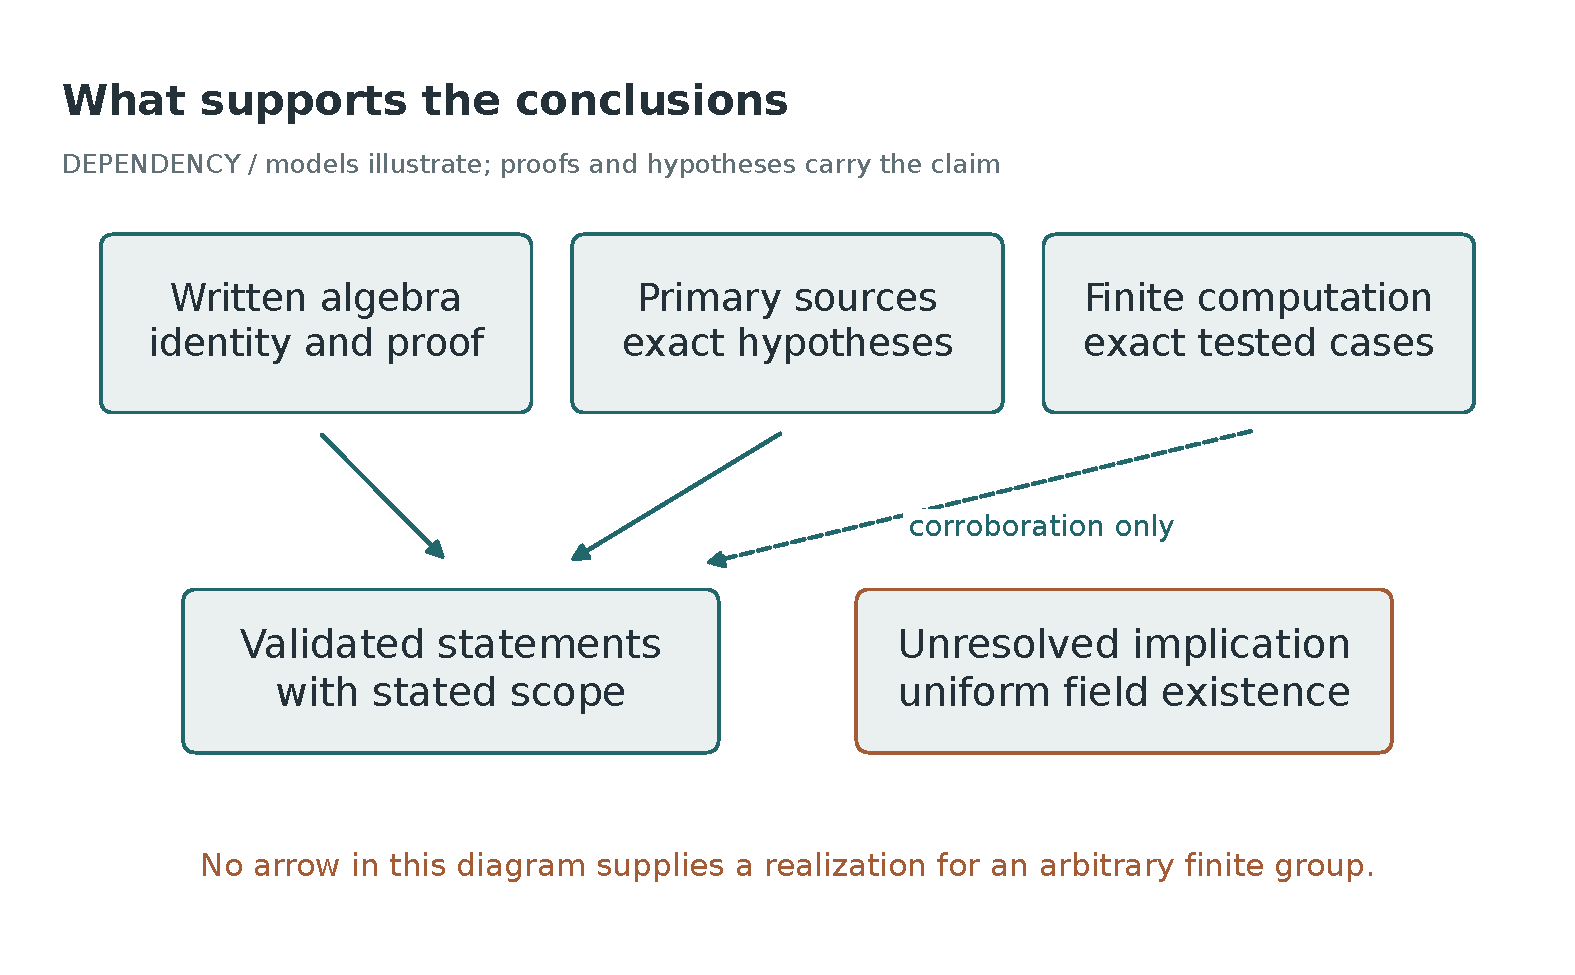
\includegraphics[width=0.94\linewidth]{../visual/figures/22_dependency.pdf}
\caption{A completed arithmetic conclusion requires an actual field and a full group argument. The generic invariant-field route and the regular-cover route reach that conclusion through their stated additional inputs. Finite matrix checks support examples and do not replace those inputs.}
\label{fig:g08-dependency}
\end{figure}

